\documentclass[uplatex, twocolumn,10pt]{jsarticle}
\和暦
\usepackage[top=25truemm,bottom=25truemm,left=25truemm,right=25truemm]{geometry}
\usepackage[dvipdfmx]{graphicx}
\usepackage{color}
\setlength{\columnsep}{3zw}

\title{ブロックチェーンプログラムの実装}
\author{744069\ 池田 敬祐}
\date{\today}

\begin{document}

\twocolumn[
  \maketitle
  \begin{abstract}
  不完全なブロックチェーンプログラムを自らの手で完成させる。完成させたプログラムを用いて実行時間の変動を計測し、ブロックチェーンの仕組みを理解する。
  \\\\
  \end{abstract}
]

\section{はじめに}
本課題では講義中に配布された不完全なブロックチェーンプログラムを完成させることを目標とする。
その後、ハッシュ値の基準(difficultyBits)を変更させた時に完成させたプログラムの実行時間がどのように変動するかを計測し、ブロックチェーン、Javaによる並列プログラミングへの理解を深めることを目的とする。

\section{実装内容の説明}
配布されたブロックチェーンプログラムの一部である「MiningNode.java」の「run()」「broadcastBlock()」「receiveMiner()」「createBlock()」「validateBlock()」「addBlockToChain()」の6つのメソッドの実装を行った。
また、実装を行うと同時にブロックチェーンプログラム全体のリファクタリングも行った。
\begin{description}
  \item[(1)]  「run()」
  \\\ \ \ 「MiningNode.java」のメインメソッド。ハッシュ値のマイニングや、Block生成、他プロセスとの通信、ブロックチェーンへのBlock追加などを行う。
  メソッドではプロセスが0(最初のプロセス)の時とそれ以外の時で処理がやや異なる。
  プロセスが0の時、ブロックチェーンの先頭のBlockを生成したのち本メソッドの機能を満たす記述を行った。
  それ以外の時、他プロセスとの通信が正確に行われる必要があった。最初にループ文を用いて通信が行われるまで次の処理に進まないように制御することで機能を満たした。
  \item[(2)]  「broadcastBlock()」
  \\\ \ \ 他プロセスにBlockを送信するメソッドである。実装済みのメソッドである「broadcastMiner()」を参考に実装を行った。
  \item[(3)]  「receiveMiner()」
  \\\ \ \ 追加したメソッド。他プロセスからMinerを受信するためのメソッドである。実装済みのメソッドである「receiveBlock()」を参考に実装を行った。
  \item[(4)]  「createBlock()」
  \\\ \ \ 新たなBlockを生成するメソッド。引数として入力されたResultなどの情報を元にBlockクラスをインスタンス化することで機能を満たしている。
  \item[(5)]  「validateBlock()」
  \\\ \ \ Blockのハッシュ値が基準を満たしているかチェックするメソッド。実装済みのメソッドである「checkHashValues()」を参考に実装を行った。
  \item[(6)]  「addBlockToChain()」
  \\\ \ \ 新しいBlockをブロックチェーンの末端に接続する。プログラムではブロックチェーンをBlockのArrayListとして実装されている。
  本メソッドではArrayListの「add()」メソッドを呼び出し、引数として入力された新しいBlockを追加することで機能を満たしている。
\end{description}

\section{実行方法}
ターミナルを開き、プログラムが存在するディレクトリに移動する。そこで、「sh javac.sh *.java」を入力し、プログラムをまとめてコンパイルする。
次に「sh java.sh Simulator -c MiningNode」を入力して実行をする。この際に「-p」オプションでプロセスを指定したり、「-t」オプションで実行時間の計測を行うことが可能である。
例えば「sh java.sh Simulator -c MiningNode -p 3 -t」と入力することでプロセス数を3として実行時間を計測しつつ実行が可能である。

\section{計測方法}
今回の計測ではプロセス数を3に固定する。ハッシュ値の基準(difficultyBits)を10から20の範囲で変更していき、それぞれの場合での実行時間を2回ずつ計測する。

\section{計測結果}
計測の結果として表1のように値が得られた。

\begin{table}[htb]
  \begin{center}
    \caption{実行時間の変動の表}
    \begin{tabular}{|r|r|r||r|} \hline
      difficultyBits & 1回目 & 2回目 & 平均 \\ \hline \hline
      20 &  &  &  \\
      19 &  &  &  \\
      18 &  &  &  \\
      17 &  &  &  \\
      16 &  &  &  \\
      15 &  &  &  \\
      14 &  &  &  \\
      13 &  &  &  \\
      12 &  &  &  \\
      11 &  &  &  \\
      10 &  &  &  \\ \hline
    \end{tabular}
  \end{center}
\end{table}

表1をグラフにしたものが図1である。

\begin{figure}
  \begin{center}
    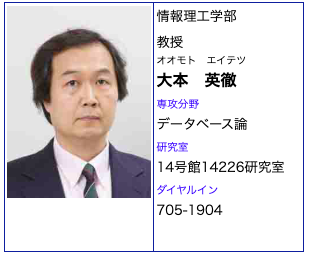
\includegraphics[width=5cm]{sample.png}
    \caption{実行時間の変動の図}
  \end{center}
\end{figure}

\section{考察}

\section{性能評価と考察}

%参考文献のリスト
\begin{thebibliography}{99}
\bibitem{tex}
D.E. クヌース,改訂新版 \TeX\ ブック,
アスキー出版局,東京,1992.
\bibitem{Nakano}
中野賢,日本語 \LaTeXe\ ブック,
アスキー出版局,東京,1996.
\end{thebibliography}


\end{document}
